\documentclass{article}
\usepackage{geometry}
\usepackage[utf8]{inputenc}
\usepackage{array}
\usepackage{tikz}
\usepackage{lipsum}
\usepgflibrary{arrows}

\geometry{
    top=10mm,
    left=5mm,
    right=5mm,
    %a5paper,
    %landscape
}

\pagenumbering{gobble}

\newcolumntype{R}[1]{>{\raggedleft\arraybackslash}p{#1}}
\newcolumntype{L}[1]{>{\raggedright\arraybackslash}p{#1}}
\newcolumntype{M}[1]{>{\centering\arraybackslash}m{#1}}

\newcommand{\kreis}{
    $\vcenter{
\begin{tikzpicture}
        \draw (0,0) circle (0.3cm);
    \end{tikzpicture}}$
}

\newcommand{\linksarrow}{
    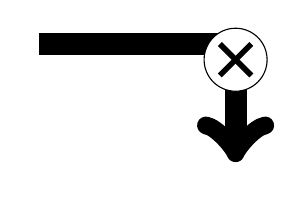
\begin{tikzpicture}
        \draw [->,line width=8] (0,1.5) -- (2.5,1.5) -- (2.5,0);
        \draw [fill=white] (2.5, 1.3) circle (0.4cm);
        \draw [line width=2] (2.3, 1.5) -- (2.7, 1.1);
        \draw [line width=2] (2.7, 1.5) -- (2.3, 1.1);
    \end{tikzpicture}
}

\newcommand{\rechtsarrow}{
    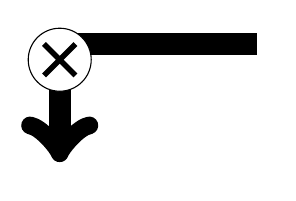
\begin{tikzpicture}
        \draw [->, line width=8] (2.5,1.5) -- (0,1.5) -- (0,0);
        \draw [fill=white] (0, 1.3) circle (0.4cm);
        \draw [line width=2] (-0.2, 1.5) -- (0.2, 1.1);
        \draw [line width=2] (-0.2, 1.1) -- (0.2, 1.5);
    \end{tikzpicture}
}

\begin{document}

\begin{center}
    \textbf{\LARGE{Stimmzettel}}\\
    \large für die Wahl des Goethopischen Parlaments\\
    und des Präsidenten\\
    am 1. Februar 2018
\end{center}

\vspace{6mm}

\begin{center}
    \textbf{\LARGE{Sie haben 2 Stimmen}}
\end{center}

\vspace{-5mm}

\begin{center}
    \begin{tabular}{R{9cm}p{.2cm}L{9cm}}
        %\linksarrow & & \rechtsarrow \\

        %\large{\textbf{hier 1 Stimme}} & & \large{\textbf{hier 1 Stimme}} \\
        %\textbf{für die Wahl} & & \textbf{für die Wahl} \\
        %\textbf{des/der Präsident/-in} & & \textbf{einer Liste (Partei)} \\[3mm]

        \linksarrow \hspace*{1mm} & & \hspace*{1mm} \rechtsarrow \\

        \large{\textbf{hier 1 Stimme}} \hspace*{3mm} & & \hspace*{3mm} \large{\textbf{hier 1 Stimme}} \\
        \textbf{für die Wahl} \hspace*{3mm} & & \hspace*{3mm} \textbf{für die Wahl} \\
        \textbf{des/der Präsident/-in} \hspace*{3mm} & & \hspace*{3mm} \textbf{einer Liste (Partei)} \\[3mm]
        \begin{tabular}[t]{|L{2mm}|L{6cm}|M{1cm}|@{}m{0pt}@{}}
            \firsthline
            1 & Schwarz, David & \kreis & \\[.5cm] \hline
            2 & Reischl, Eric & \kreis & \\[.5cm] \hline
            3 & Pompei, Paula-Francesca & \kreis & \\[.5cm] \hline
            4 & Aylin Bozcali & \kreis & \\[.5cm] \hline
        \end{tabular}
        & &
        \begin{tabular}[t]{|M{1cm}|L{6cm}|m{2mm}|@{}m{0pt}@{}}
            \firsthline
            \kreis & Partei für Gleichberechtigung (PfG) & 1 & \\[.5cm] \hline
            \kreis & Minderheitengremium (MIG) & 2 & \\[.5cm] \hline
            \kreis & Kleine Kätzchen Partei (KKP) & 3 & \\[.5cm] \hline
            \kreis & Einheitliche Arbeiterpartei (EAP) & 4 & \\[.5cm] \hline
            \kreis & Sozialliberale Demokraten (SLD) & 5 & \\[.5cm] \hline
            \kreis & Kommunistisch Altruistische Partei (Ktkat) & 6 & \\[.5cm] \hline
            \kreis & Goethopische Gerechtigkeitspartei (GGP) & 7 & \\[.5cm] \hline
            \kreis & Die Blauen (DB) & 8 & \\[.5cm] \hline
            \kreis & Die Goethopia Partei (DGP) & 9 & \\[.5cm] \hline
        \end{tabular}
        \\
    \end{tabular}

\end{center}

\end{document}
